\documentclass[11pt,class=report,crop=false]{standalone}
\usepackage[screen]{../mathgame}

%\usepackage{siunitx}
%\sisetup{locale = FR,detect-all,per-mode = symbol}

\begin{document}

%====================================================================
\chapitre{Fractales}
%====================================================================


\insertvideo{nfDxFGE1CbU}{partie 17.1. Montagnes}

\insertvideo{rpUqm1vYaf8}{partie 17.2. IFS}

\insertvideo{Ykz_qhq8q0o}{partie 17.3. L-systèmes (2D)}

\insertvideo{hMB_hDqel28}{partie 17.4. L-systèmes (3D)}


\objectifs{
Les fractales sont des formes géométriques auto-similaires : lorsque l'on zoome sur une partie, on retrouve une image ressemblant à la figure globale. Les structures fractales permettent de dessiner des paysages et de la végétation. La méthode est facile à implémenter, permet de générer aléatoirement une grande variété de structures, utilise très peu de données, mais par contre nécessite des calculs.}


\medskip

\objectifs{Dans ce chapitre on se contente d'une modélisation assez grossière : sans couleur ni texture.}

\index{fractale}

%%%%%%%%%%%%%%%%%%%%%%%%%%%%%%%%%%%%%%%%%%%%%%%%%%%%%%%%%%%%%%%%%%%%%
\section{Montagnes}

Dessinons un paysage avec des montagnes et des vallées. La génération est rapide, aléatoire et paramétrable.

Afin de mieux comprendre l'algorithme général, on commence avec une seule dimension par la génération du profil d'une montagne, ou bien d'un cours de bourse.

%--------------------------------------------------------------------
\subsection{Une dimension}


\begin{center}
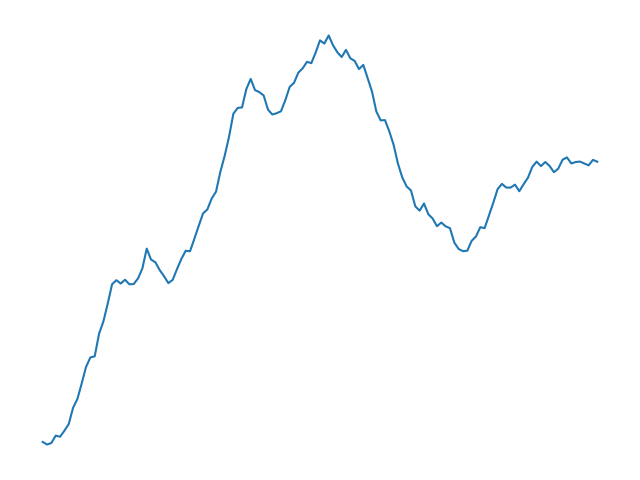
\includegraphics[scale=\myscale,scale=0.4]{figures/landscape-01}
\end{center}


\textbf{Données.} Voici les données qui permettent de générer un profil de montagne :

\begin{itemize}
  \item une altitude de départ $H_a$,
  \item une altitude d'arrivée $H_b$, 
  \item une valeur d'amplitude maximale $h_0$,
  \item un coefficient de rugosité $r$,
  \item un nombre de subdivisions $N = 2^n$.
\end{itemize}

On peut aussi fixer le germe (\emph{seed}) du processus de génération pseudo-aléatoire afin de pouvoir reproduire les mêmes résultats lors d'une génération future.

\medskip

\textbf{Sortie.}
L'algorithme renvoie $N+1$ valeurs (la première étant $H_a$ et la dernière $H_b$).


\begin{center}
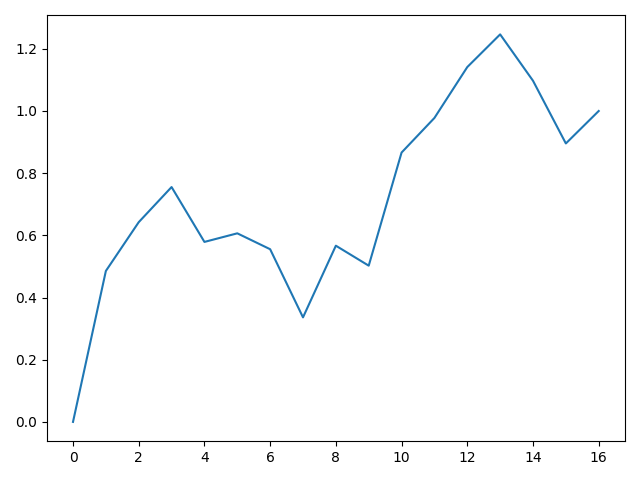
\includegraphics[scale=\myscale,scale=0.5]{figures/landscape-02}

\nopagebreak

\begin{minipage}{0.8\textwidth}
\center\emph{
Un exemple avec $n=5$, $N=16$, $H_a=0$, $H_b=1$, $h_0=1$ et $r=0.7$.}
\end{minipage}

\end{center}

\medskip



\textbf{Algorithme.}

On considère qu'on trace le profil au-dessus d'un segment $[a,b]$.
L'algorithme est un calcul de moyenne des altitudes avec ajout d'un saut aléatoire.
Il s'effectue par dichotomies successives de l'intervalle de départ.

\begin{itemize}
  \item \emph{Étape $1$.} En $c=\frac{a+b}{2}$, qui est le milieu de $[a,b]$, on calcule la moyenne des hauteurs de départ et d'arrivée à laquelle on ajoute une valeur aléatoire :
$$H_c = \frac{H_a+H_b}{2} + v.$$
La valeur $v$ est tirée aléatoirement dans l'intervalle $[-h_0,+h_0]$.
On obtient donc $3$ ($=2^1+1$) valeurs $H_a,H_c,H_b$.

\myfigure{0.8}{
	\tikzinput{fig-montagne-01}
} 


  \item \emph{Étape $2$.} On recommence entre $a$ et $c$ en calculant la moyenne entre $H_a$ et $H_c$ à laquelle on ajoute une valeur aléatoire de $[-h_1,+h_1]$ où $h_1 = \frac{h_0}{2^r}$. On fait de même entre $c$ et $b$, avec la moyenne entre $H_c$ et $H_b$ et une nouvelle valeur aléatoire de $[-h_1,+h_1]$. On obtient $5$ ($=2^2+1$) altitudes.

\myfigure{0.8}{
	\tikzinput{fig-montagne-02}
} 



  \item \emph{...}
  \item \emph{Étape $i$.} On obtient $2^i+1$ altitudes. La hauteur aléatoire est choisie dans $[-h_i,+h_i]$ où $h_i = \frac{h_0}{2^{ir}}$.

  \item \emph{Étape $n$.} On obtient $2^n+1$ altitudes. 
\end{itemize}

\begin{exemple}
Voici le déroulé de la construction étape par étape.


\begin{center}
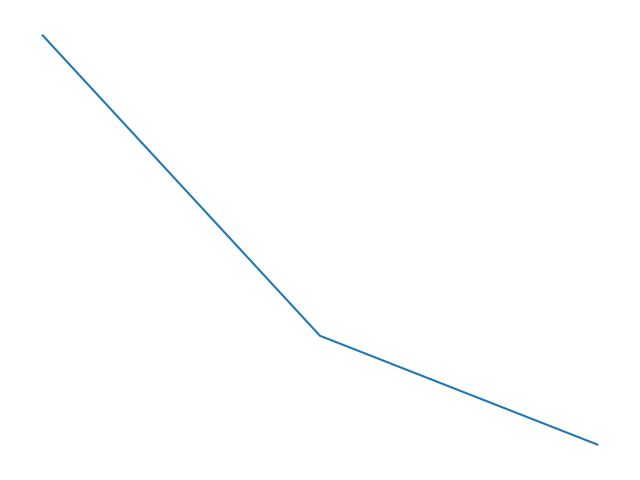
\includegraphics[scale=\myscale,scale=0.2]{figures/landscape-03-1}
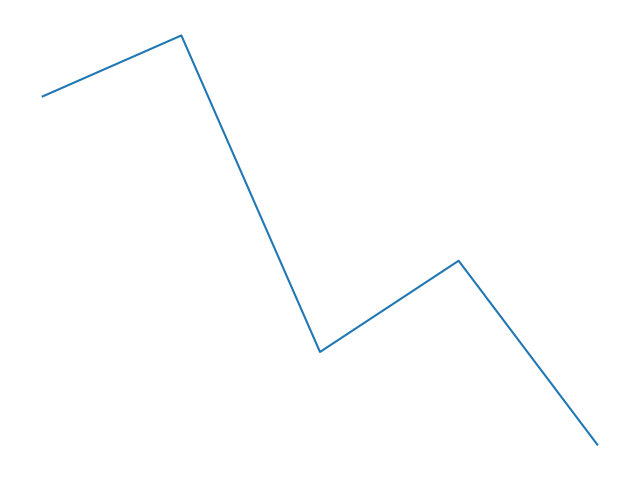
\includegraphics[scale=\myscale,scale=0.2]{figures/landscape-03-2}
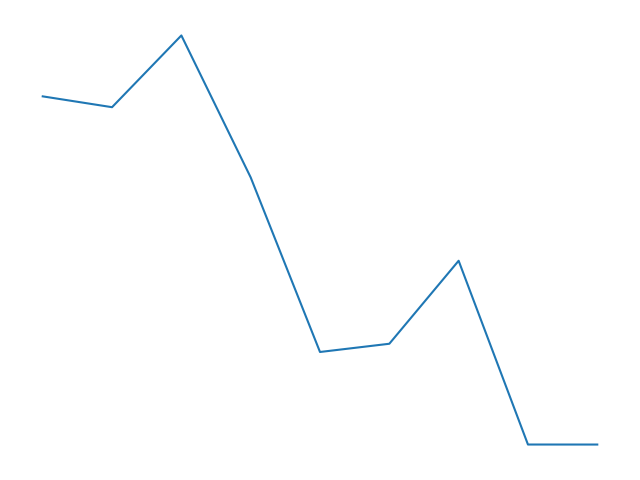
\includegraphics[scale=\myscale,scale=0.2]{figures/landscape-03-3}
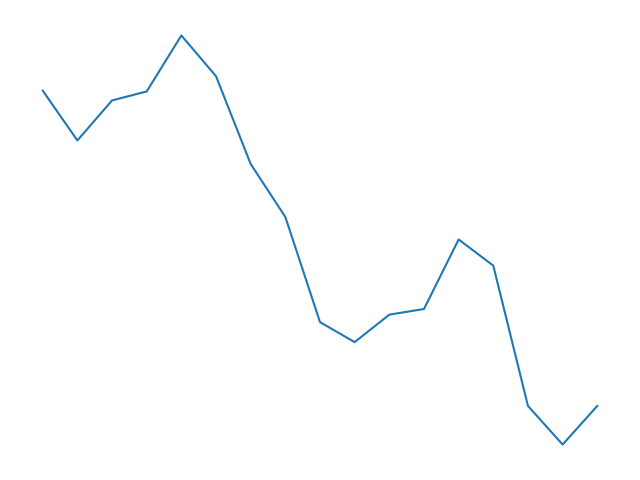
\includegraphics[scale=\myscale,scale=0.2]{figures/landscape-03-4}

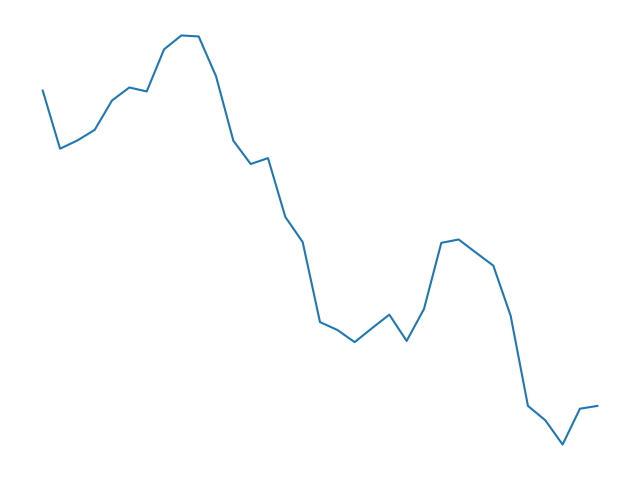
\includegraphics[scale=\myscale,scale=0.2]{figures/landscape-03-5}
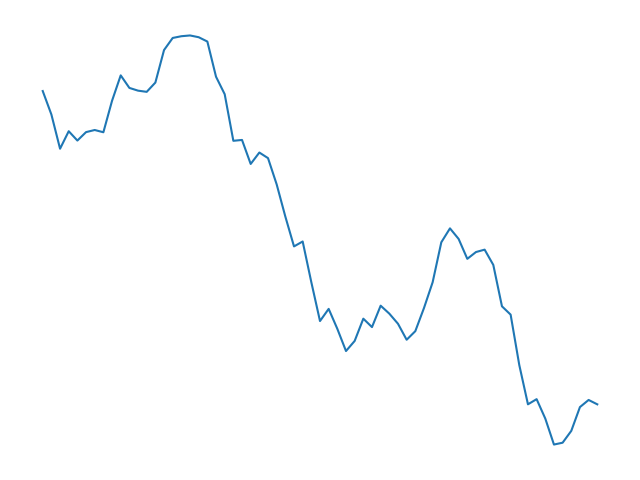
\includegraphics[scale=\myscale,scale=0.2]{figures/landscape-03-6}
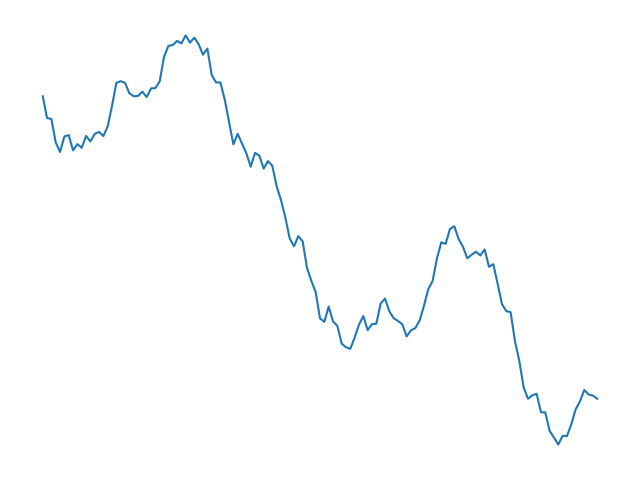
\includegraphics[scale=\myscale,scale=0.2]{figures/landscape-03-7}
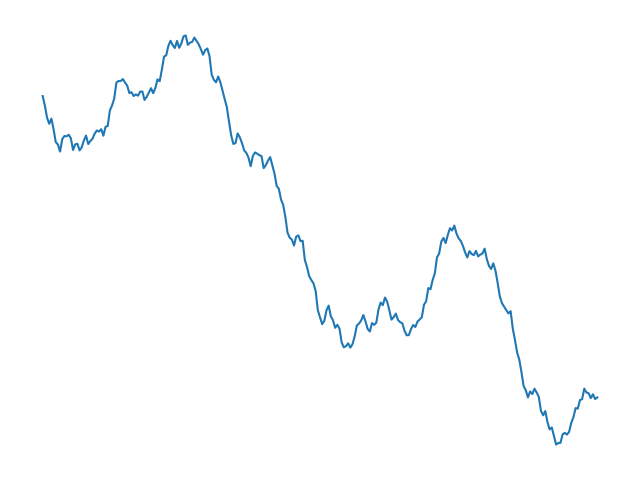
\includegraphics[scale=\myscale,scale=0.2]{figures/landscape-03-8}

\nopagebreak

\begin{minipage}{0.8\textwidth}
\center\emph{
Les étapes de la construction avec $n$ variant de $1$ à $8$.}
\end{minipage}

\end{center}


\end{exemple}

\begin{exemple}
Voici les profils obtenus pour différents tirages aléatoires. Les valeurs $H_a$, $H_b$, $h_0$ et $r$ sont les mêmes pour tous ces profils.

\begin{center}
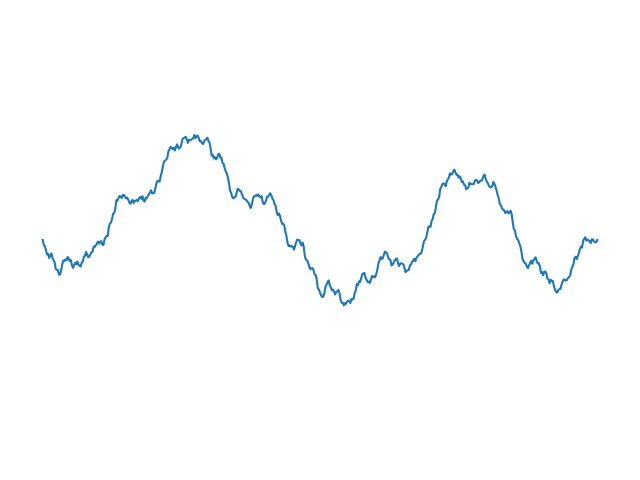
\includegraphics[scale=\myscale,scale=0.3]{figures/landscape-04-1}
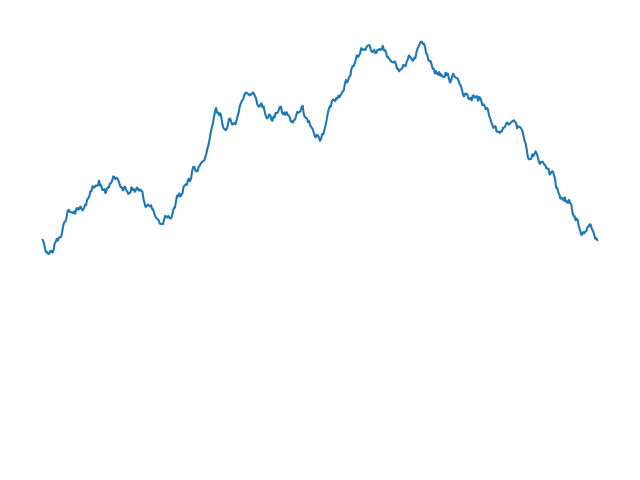
\includegraphics[scale=\myscale,scale=0.3]{figures/landscape-04-6}
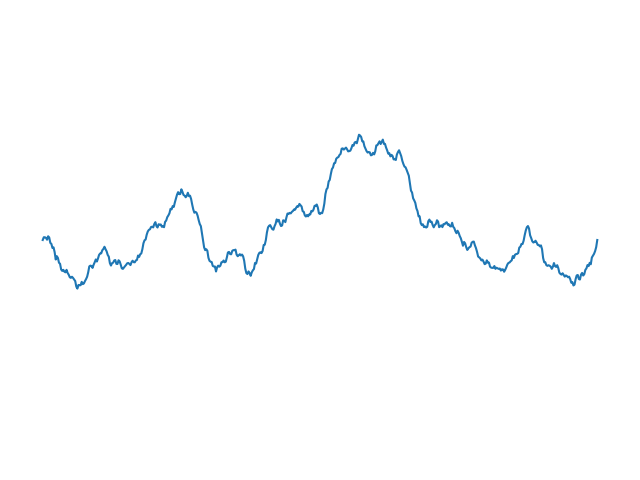
\includegraphics[scale=\myscale,scale=0.3]{figures/landscape-04-3}

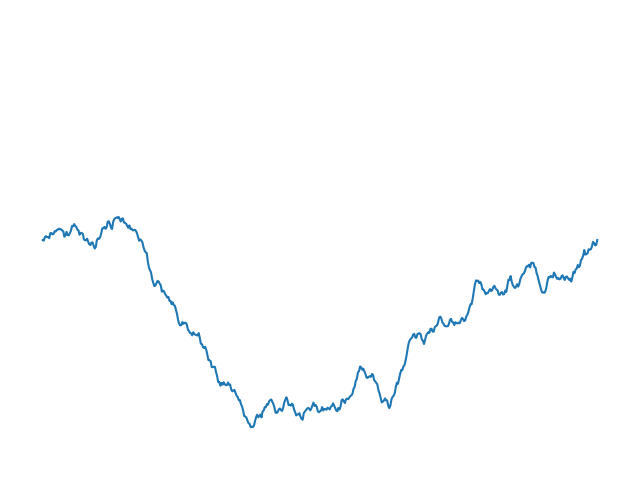
\includegraphics[scale=\myscale,scale=0.3]{figures/landscape-04-4}
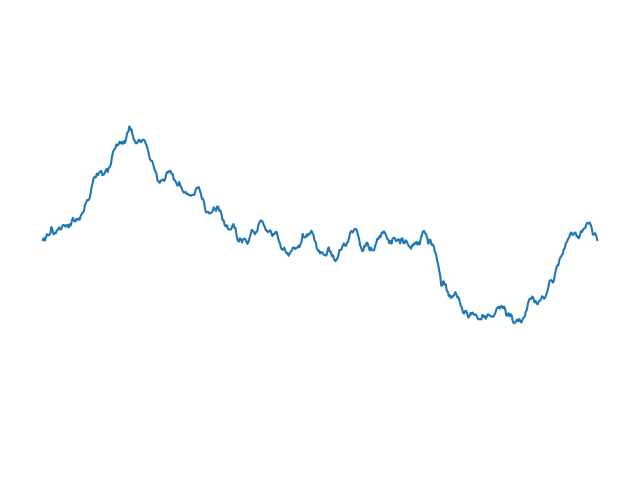
\includegraphics[scale=\myscale,scale=0.3]{figures/landscape-04-2}
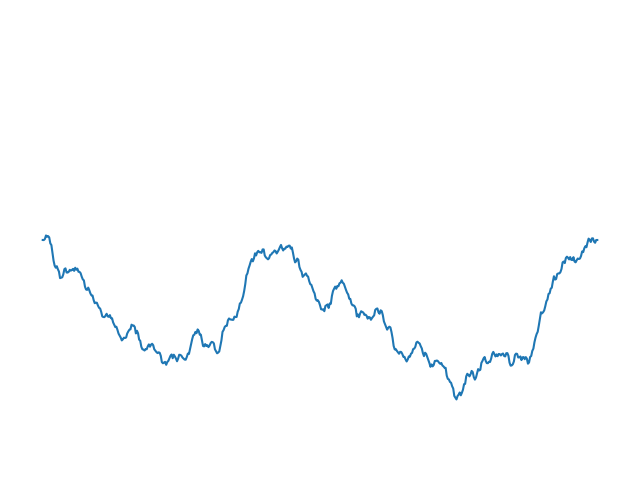
\includegraphics[scale=\myscale,scale=0.3]{figures/landscape-04-5}
\end{center}

\end{exemple}

\begin{exemple}
Voici les profils obtenus pour différentes valeurs de l'amplitude $h_0$. 
Les autres valeurs (y compris le germe du tirage pseudo-aléatoire) sont les mêmes.

\begin{center}
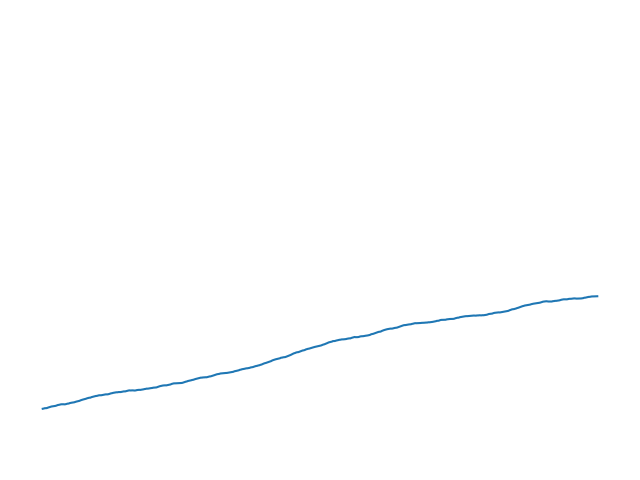
\includegraphics[scale=\myscale,scale=0.2]{figures/landscape-05-01}
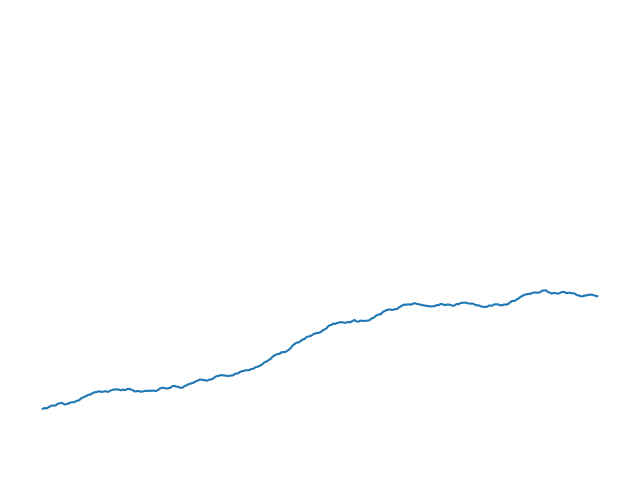
\includegraphics[scale=\myscale,scale=0.2]{figures/landscape-05-03}
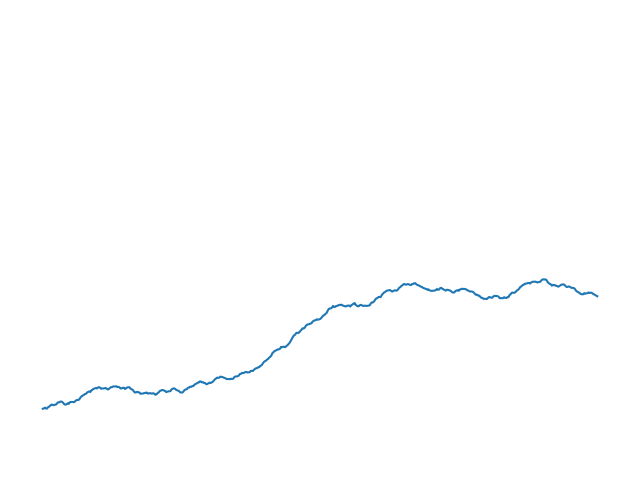
\includegraphics[scale=\myscale,scale=0.2]{figures/landscape-05-05}
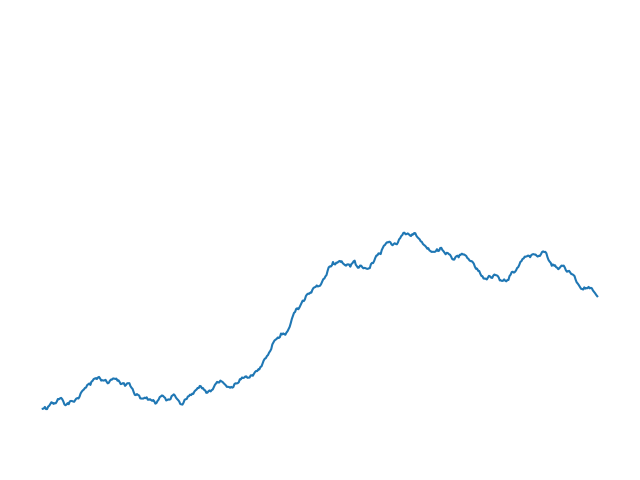
\includegraphics[scale=\myscale,scale=0.2]{figures/landscape-05-10}

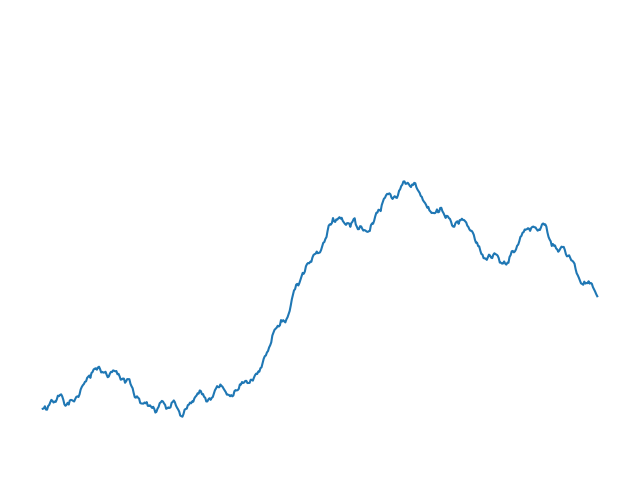
\includegraphics[scale=\myscale,scale=0.2]{figures/landscape-05-15}
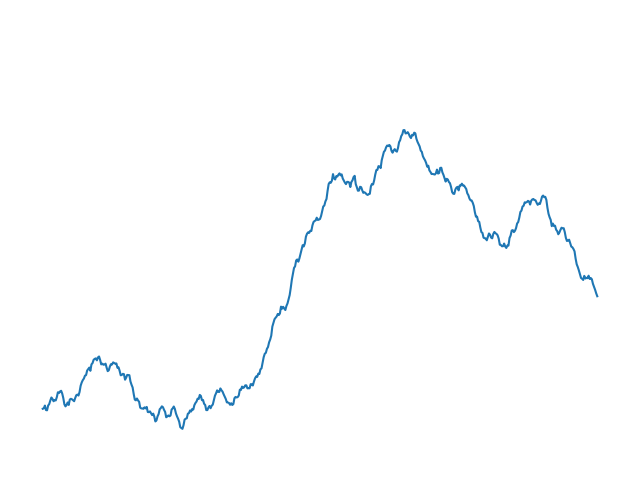
\includegraphics[scale=\myscale,scale=0.2]{figures/landscape-05-20}
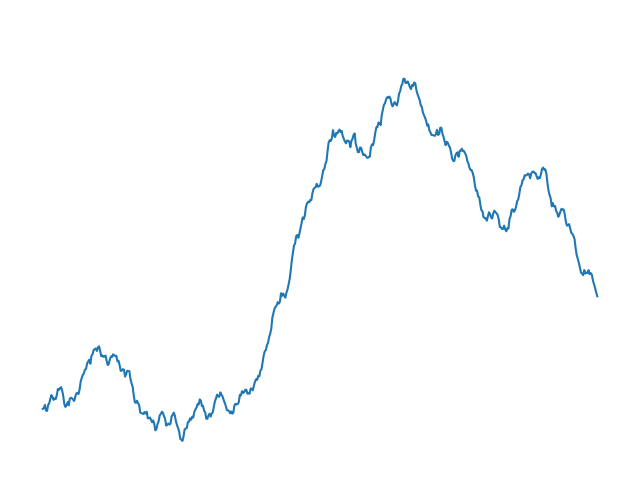
\includegraphics[scale=\myscale,scale=0.2]{figures/landscape-05-25}
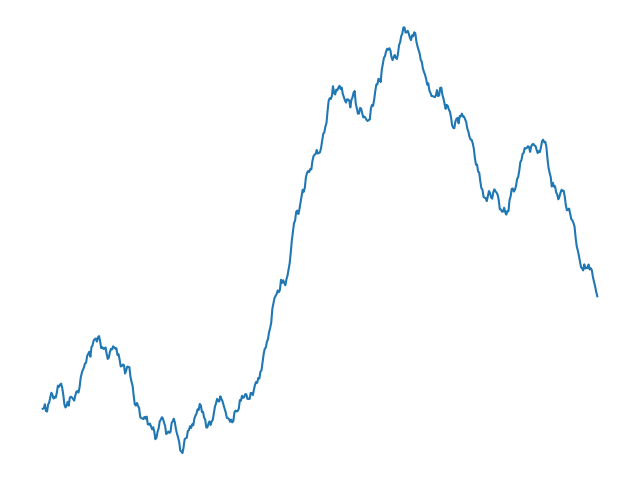
\includegraphics[scale=\myscale,scale=0.2]{figures/landscape-05-30}

\nopagebreak

\begin{minipage}{0.8\textwidth}
\center\emph{
L'amplitude de variation aléatoire $h_0$ varie : $0.1$, $0.3$, $0.5$, $1.0$, $1.5$, $2.0$, $2.5$, $3.0$.}
\end{minipage}

\end{center}

\end{exemple}

\begin{exemple}
Voici les profils obtenus pour différentes valeurs de la rugosité $r$. 
Les autres valeurs (y compris le germe du tirage pseudo-aléatoire) sont les mêmes. Plus le coefficient $r$ est grand, plus la courbe est lisse.

\begin{center}
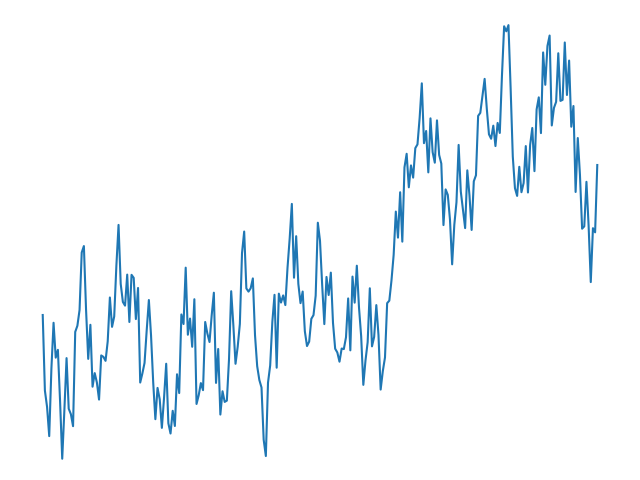
\includegraphics[scale=\myscale,scale=0.2]{figures/landscape-06-02}
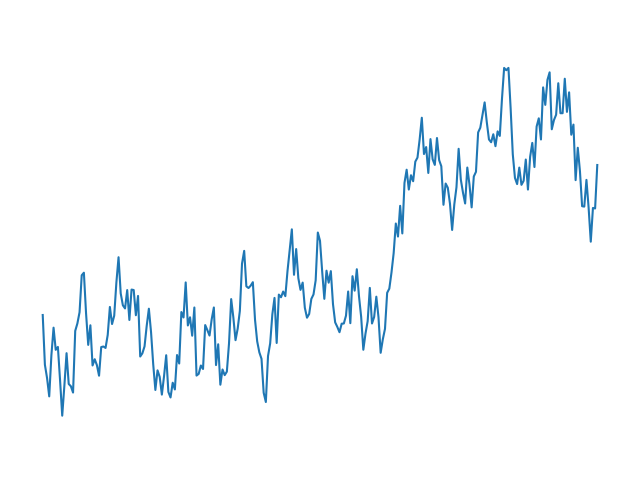
\includegraphics[scale=\myscale,scale=0.2]{figures/landscape-06-03}
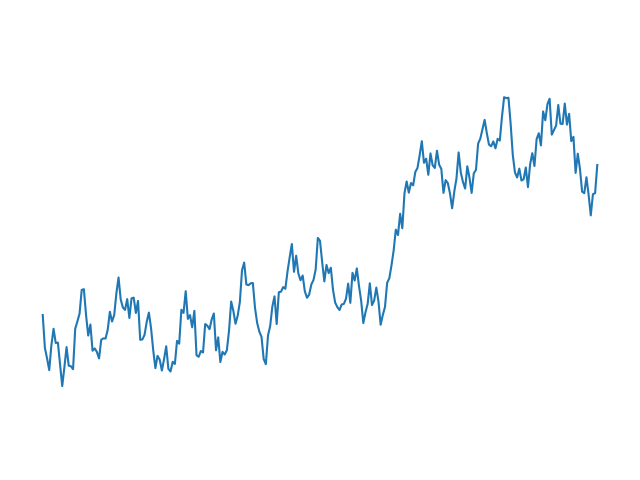
\includegraphics[scale=\myscale,scale=0.2]{figures/landscape-06-04}
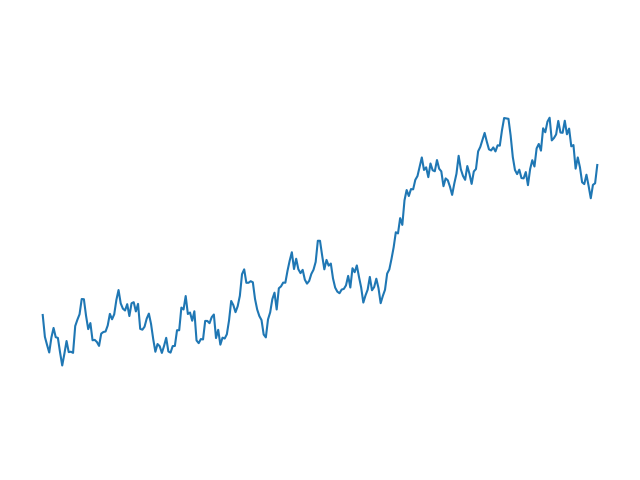
\includegraphics[scale=\myscale,scale=0.2]{figures/landscape-06-05}

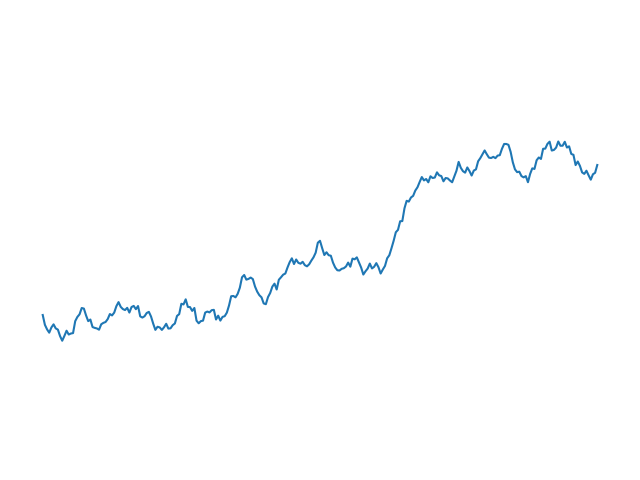
\includegraphics[scale=\myscale,scale=0.2]{figures/landscape-06-07}
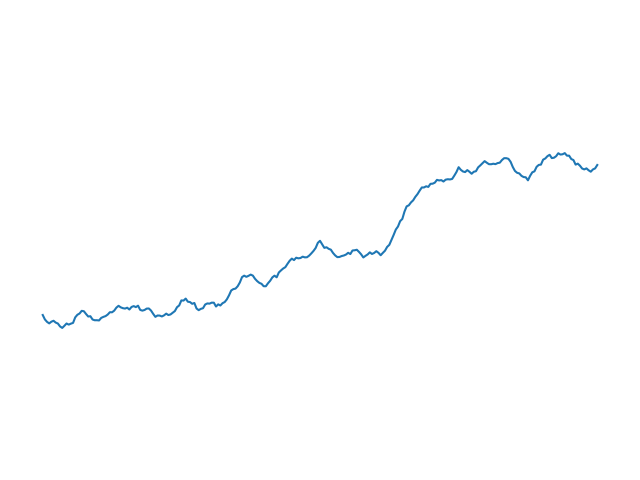
\includegraphics[scale=\myscale,scale=0.2]{figures/landscape-06-09}
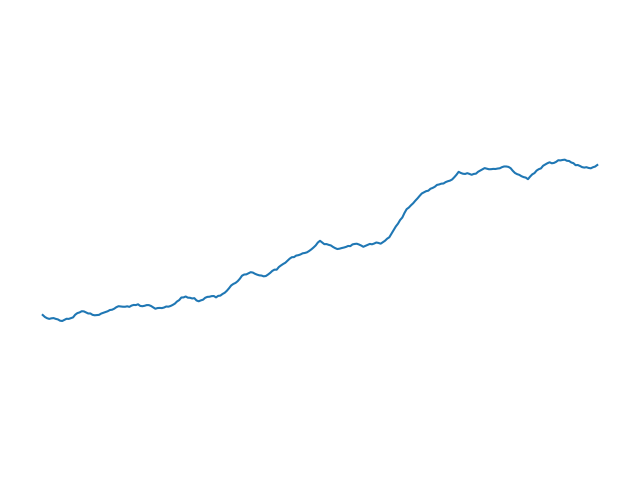
\includegraphics[scale=\myscale,scale=0.2]{figures/landscape-06-11}
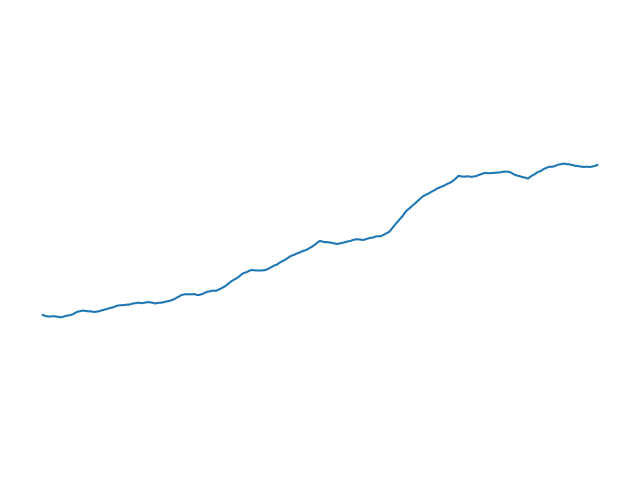
\includegraphics[scale=\myscale,scale=0.2]{figures/landscape-06-13}

\nopagebreak

\begin{minipage}{0.8\textwidth}
\center\emph{
Le coefficient de rugosité $r$ varie : $0.2$, $0.3$, $0.4$, $0.5$, $0.7$, $0.9$, $1.1$, $1.3$.}
\end{minipage}

\end{center}

\end{exemple}


\begin{exercicecours}
Programmer cet algorithme sous la forme itérative comme expliqué ci-dessus. Programmer aussi une version récursive.
\end{exercicecours}

%--------------------------------------------------------------------
\subsection{Deux dimensions}

Tracer une surface dans l'espace qui représente un paysage est évidemment la situation qui nous intéresse le plus. Il s'agit d'adapter l'algorithme précédent avec une dimension supplémentaire afin de générer les altitudes d'un terrain.


\textbf{Données.} 
Voici les données qui permettent de générer un profil de montagne au-dessus d'une zone carrée :

\begin{itemize}
  \item une altitude de départ $H$ qui sera l'altitude aux quatre coins du carré,
  \item une valeur d'amplitude maximale $h_0$,
  \item un coefficient de rugosité $r$,
  \item un nombre de subdivisions $N = 2^n$.
\end{itemize}
\medskip

\textbf{Sortie.}
L'algorithme renvoie $(N+1)^2$ valeurs, correspondant aux altitudes au-dessus d'une grille carrée $(N+1) \times (N+1)$.


\begin{center}
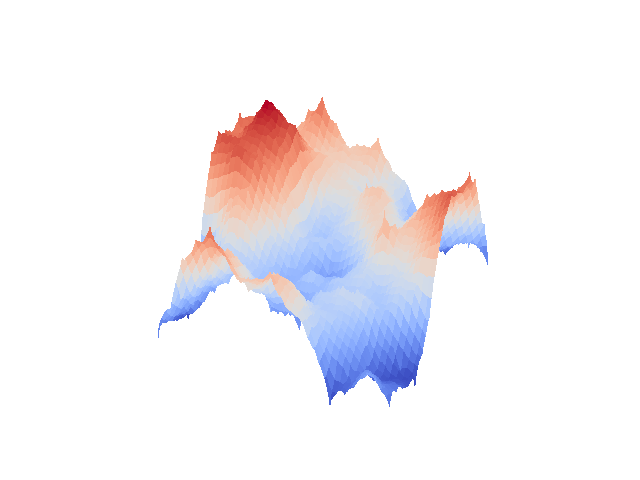
\includegraphics[scale=\myscale,scale=0.5]{figures/hauteurs-02}
\end{center}

\medskip



\textbf{Algorithme.}

La construction se fait en itérant une construction \og{}diamant-carré\fg{}.

\begin{itemize}

  \item \emph{Étape diamant.} 
  À partir de $4$ valeurs connues aux sommets d'un carré, on détermine une valeur au centre selon la formule :
  $$\text{moyenne des $4$ valeurs} \ + \ \text{ valeur aléatoire}.$$
  À l'étape numéro $i$ la valeur aléatoire est dans l'intervalle $[-h_i,+h_i]$ où $h_i = \frac{h_0}{2^{ir}}$.


\myfigure{0.8}{
	\tikzinput{fig-montagne-03}
} 



  \item \emph{Étape carré.}
  À partir de $4$ valeurs connues aux sommets d'un losange, on détermine une valeur au centre selon la formule :
  $$\text{moyenne des $4$ valeurs} \ + \ \text{ valeur aléatoire}.$$
  À l'étape numéro $i$ la valeur aléatoire est de nouveau choisie dans l'intervalle $[-h_i,+h_i]$.

\myfigure{0.8}{
	\tikzinput{fig-montagne-04}
} 


\end{itemize}

L'étape carré est en fait une étape diamant composée avec une rotation de \ang{45}.

Il y a un problème avec l'étape carré car, aux bords de la zone carrée initiale, on ne dispose pas d'un losange complet et donc on n'a pas toujours $4$ valeurs à moyenner. Plusieurs solutions sont possibles :
\begin{itemize}
  \item ne tenir compte que des sommets présents en faisant la moyenne sur $3$ sommets au lieu de $4$ ;
  \item considérer que les valeurs sont périodiques : les valeurs du côté gauche du tableau initial sont les mêmes que les valeurs du côté droit, et les valeurs du bas sont les mêmes que les valeurs du haut.
\end{itemize}

\myfigure{0.6}{
	\tikzinput{fig-montagne-06}
} 

Nous adoptons la seconde solution qui a l'avantage de créer une surface avec le bord gauche identique au bord droit et le bord haut identique à celui du bas et donne ainsi un motif de base qui se recolle parfaitement lorsque qu'on en juxtapose plusieurs.


Voici les points où les altitudes sont calculées lors des premières étapes de la construction \og{}diamant-carré\fg{}.

\myfigure{0.5}{
	\tikzinput{fig-montagne-05a}\qquad
	\tikzinput{fig-montagne-05b}\qquad
	\tikzinput{fig-montagne-05c}
}

\myfigure{0.5}{	
	\tikzinput{fig-montagne-05d}\qquad
	\tikzinput{fig-montagne-05e}
} 




\begin{exemple}
Voici un exemple de cette construction étape par étape.


\begin{center}
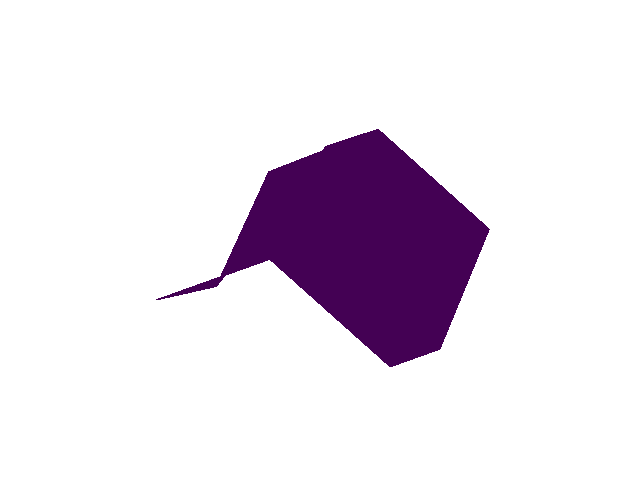
\includegraphics[scale=\myscale,scale=0.3]{figures/diamant-carre-01-1}
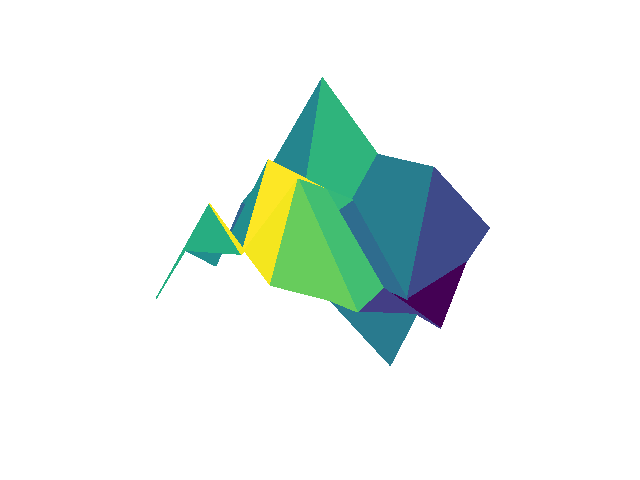
\includegraphics[scale=\myscale,scale=0.3]{figures/diamant-carre-01-2}
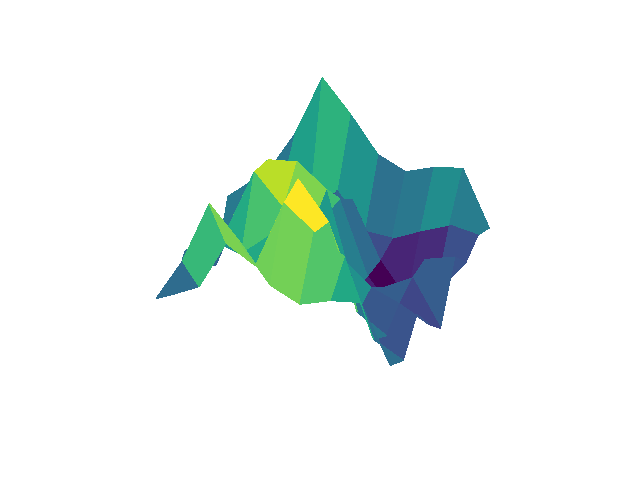
\includegraphics[scale=\myscale,scale=0.3]{figures/diamant-carre-01-3}

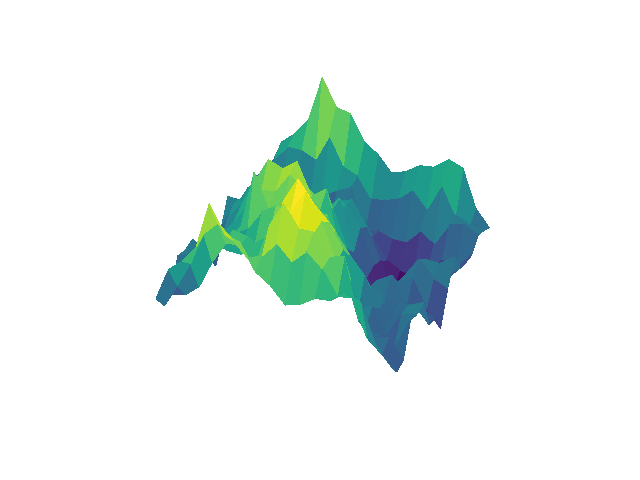
\includegraphics[scale=\myscale,scale=0.3]{figures/diamant-carre-01-4}
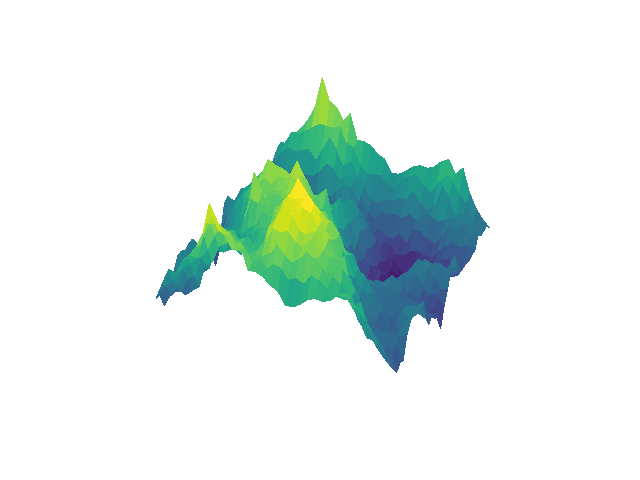
\includegraphics[scale=\myscale,scale=0.3]{figures/diamant-carre-01-5}
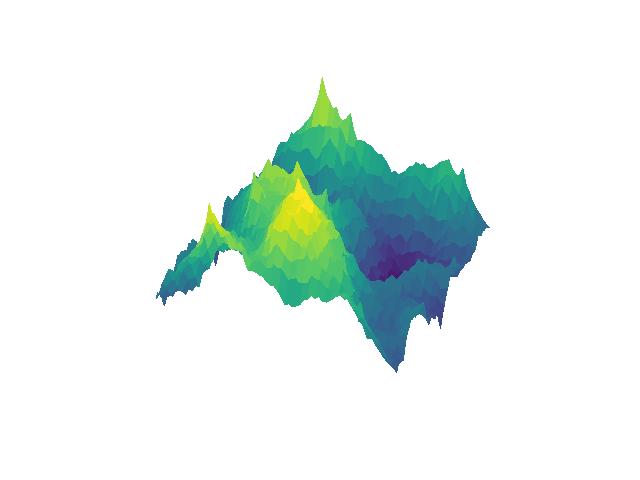
\includegraphics[scale=\myscale,scale=0.3]{figures/diamant-carre-01-6}


\nopagebreak

\begin{minipage}{0.8\textwidth}
\center\emph{
Les étapes de la construction avec $n$ variant de $1$ à $6$.}
\end{minipage}

\end{center}


\end{exemple}


\begin{exemple}
Voici les profils obtenus pour différents tirages aléatoires et différentes valeurs des paramètres.

\begin{center}
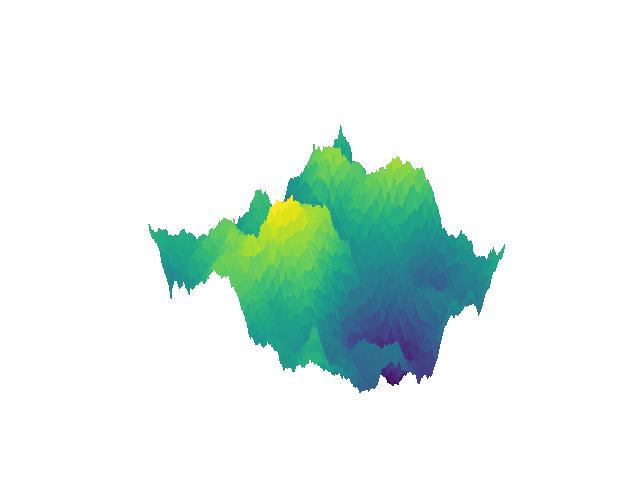
\includegraphics[scale=\myscale,scale=0.3]{figures/diamant-carre-02-1}
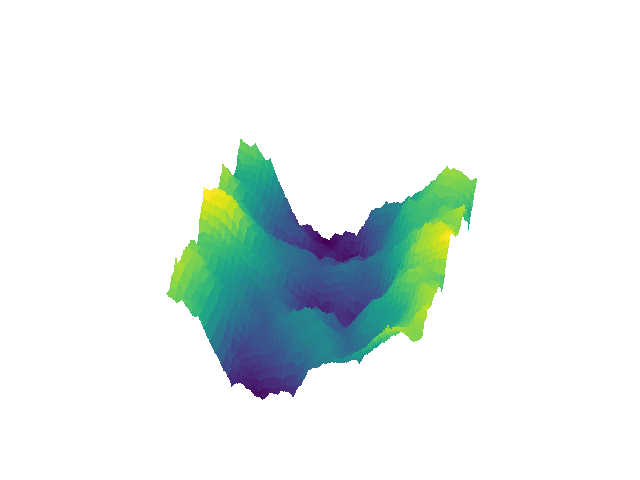
\includegraphics[scale=\myscale,scale=0.3]{figures/diamant-carre-02-2}
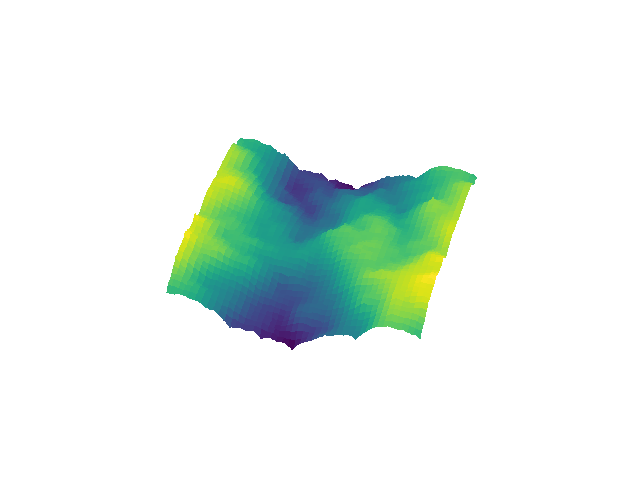
\includegraphics[scale=\myscale,scale=0.3]{figures/diamant-carre-02-3}

\end{center}

\end{exemple}

\textbf{Carte de hauteurs -- \emph{heightmap}.}

Comment utiliser les surfaces obtenues ? 
Tout d'abord les données produites se résument à un tableau de taille $(N+1)\times(N+1)$ où chaque entrée en $(i,j)$ est un nombre réel représentant l'altitude du terrain au-dessus du point $(i,j)$.
Les données se transforment aisément en une image en niveaux de gris, appelée \defi{carte de hauteurs} (\defi{heightmap}), sa taille est $(N+1)\times(N+1)$ et chaque niveau de gris représente une hauteur mise à l'échelle et arrondie. Par exemple $0$ (noir) pour l'altitude la plus basse et $255$ (blanc) pour l'altitude la plus haute.

Cette image peut ensuite être importée dans un logiciel de traitement d'images (par exemple \textsl{Blender}) pour reconstituer le paysage et obtenir un rendu 3D avec éclairage, texture...

\begin{exemple}
Construction d'une carte de hauteurs et rendu 3D.

\begin{center}

\begin{minipage}{0.4\textwidth}
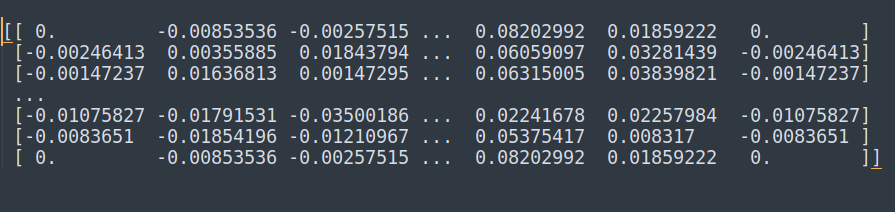
\includegraphics[scale=\myscale,scale=0.2]{figures/hauteurs-capture-04}
\end{minipage}
\begin{minipage}{0.4\textwidth}
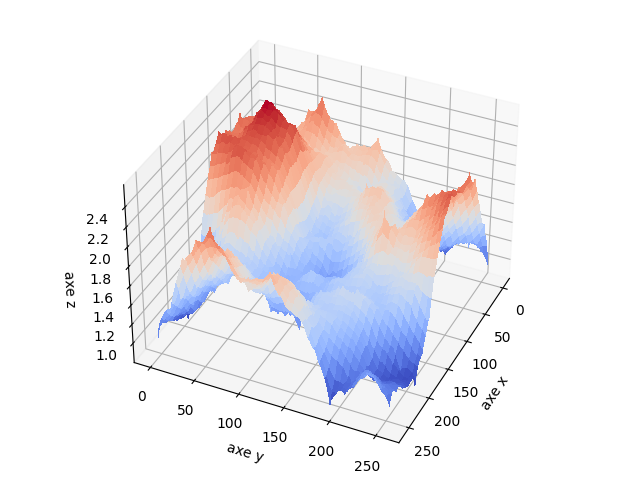
\includegraphics[scale=\myscale,scale=0.5]{figures/hauteurs-01}
\end{minipage}

\begin{minipage}{0.4\textwidth}
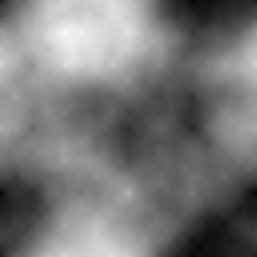
\includegraphics[scale=\myscale,scale=0.5]{figures/hauteurs-03}
\end{minipage}
\begin{minipage}{0.5\textwidth}
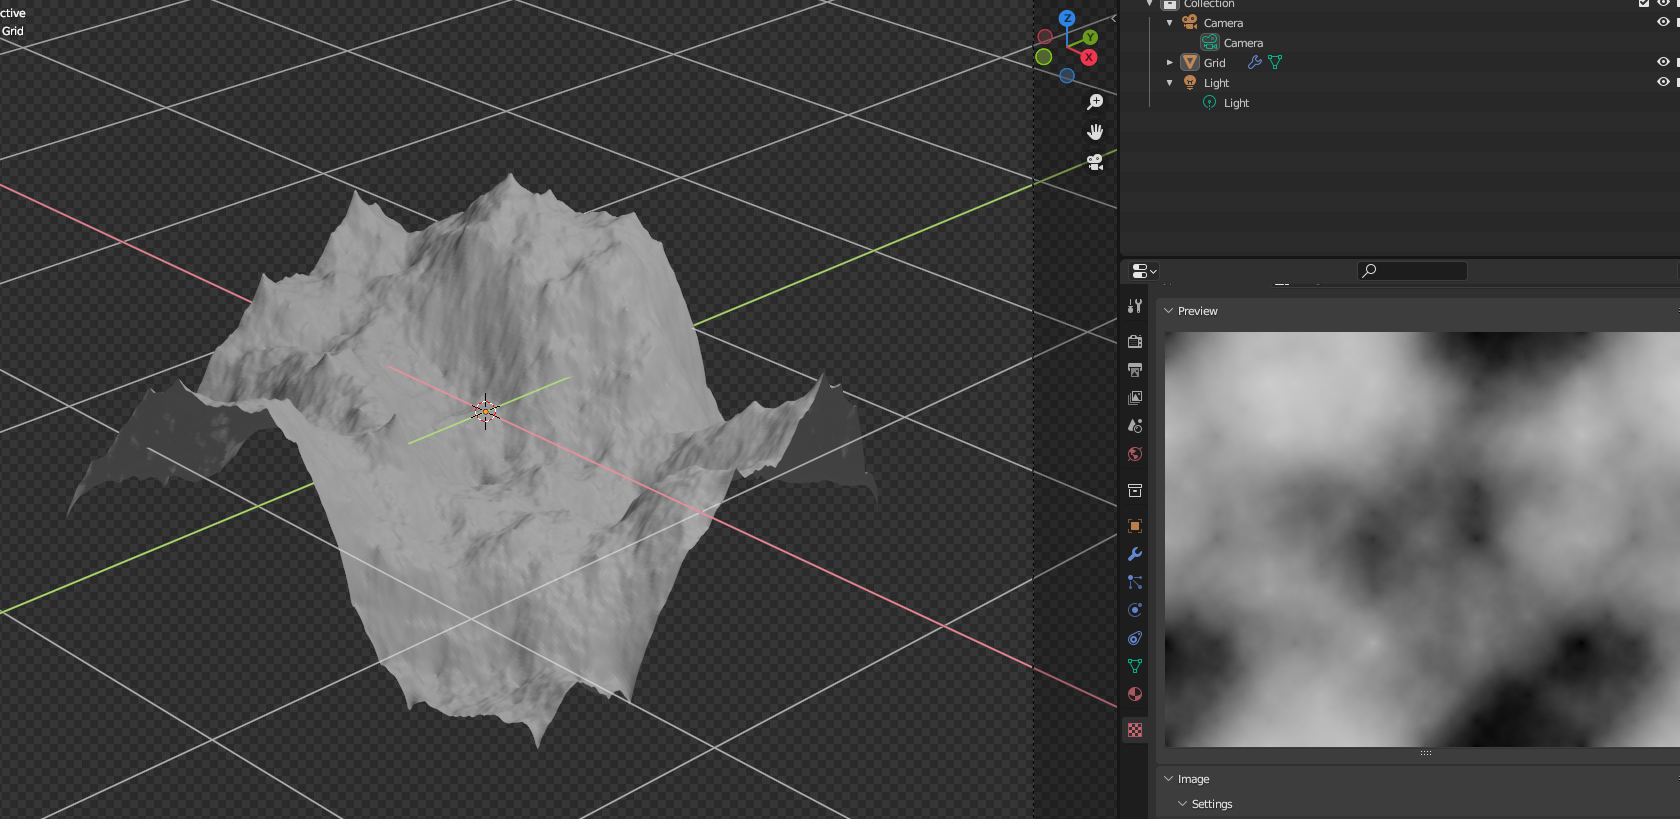
\includegraphics[scale=\myscale,scale=0.15]{figures/hauteurs-capture-new-02}
\end{minipage}

\smallskip

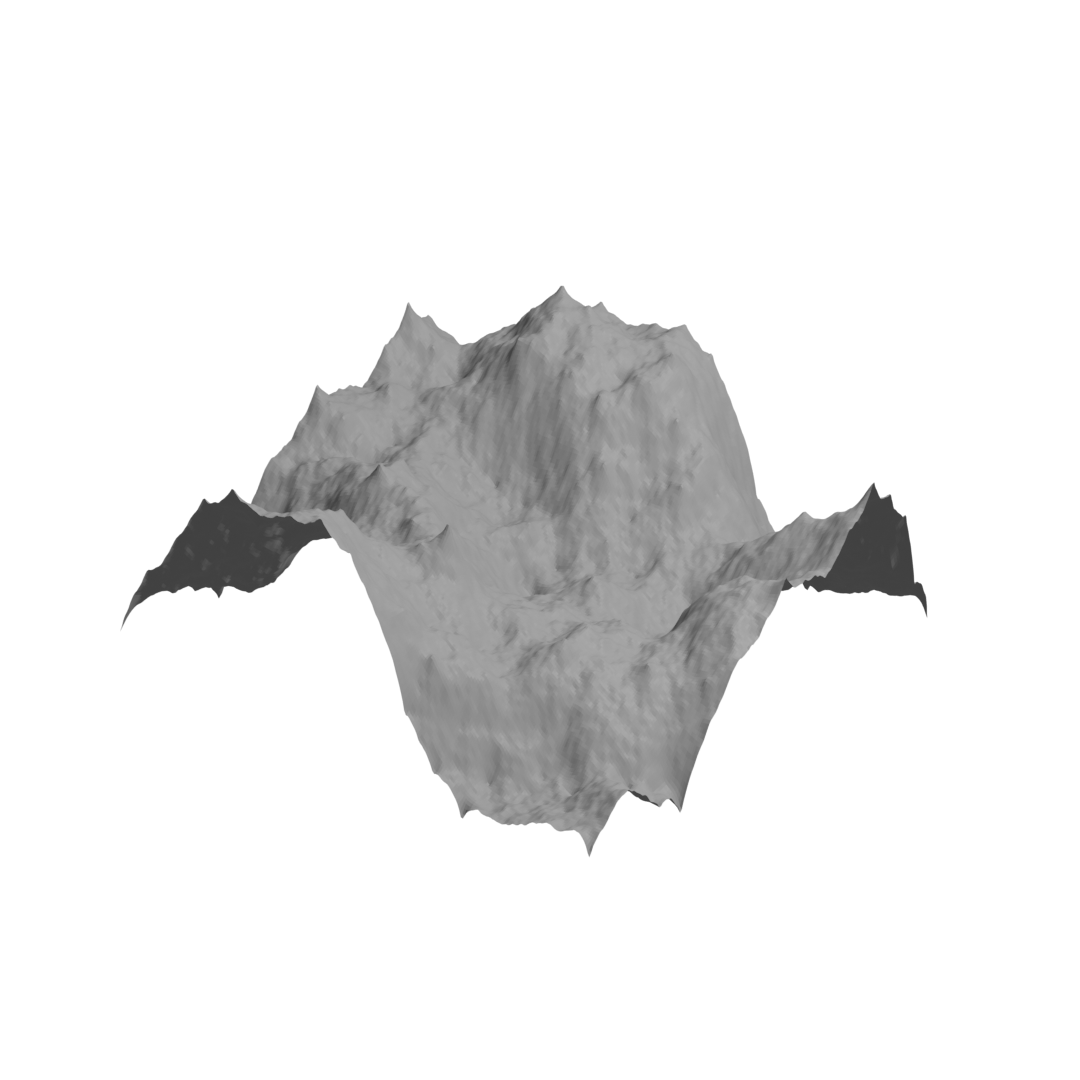
\includegraphics[scale=\myscale,scale=0.25]{figures/hauteurs-render-new-01}

\smallskip

\nopagebreak

\begin{minipage}{0.8\textwidth}
\center\emph{
(a) Le tableau des hauteurs. 
(b) La visualisation \Python{} avec \matplotlib.
(c) Carte des hauteurs c-à-d l'image en niveaux de gris.
(d) Reconstitution de la surface dans \textsl{Blender}.
(e) Rendu 3D.}
\end{minipage}

\end{center}


\end{exemple}




\textbf{Niveau de la mer.}

On peut créer un paysage de bord de mer : tout ce qui a une hauteur négative est ramené à l'altitude $0$ par la formule $h'= \max(h,0)$. Dans la pratique on fixe le niveau de l'eau à une altitude $h_e$ et on applique la formule :
$$h' = \max(h,h_e)$$
qui conserve la hauteur $h$ si on est au-dessus de la mer et ramène l'altitude à $h_e$ sinon.

\begin{exemple}
Voici le changement de paysage lorsque le niveau de l'eau monte.

\begin{center}
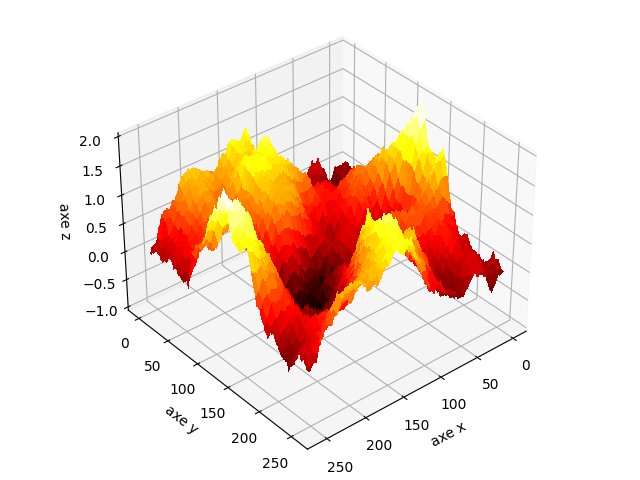
\includegraphics[scale=\myscale,scale=0.4]{figures/diamant-carre-03-1}
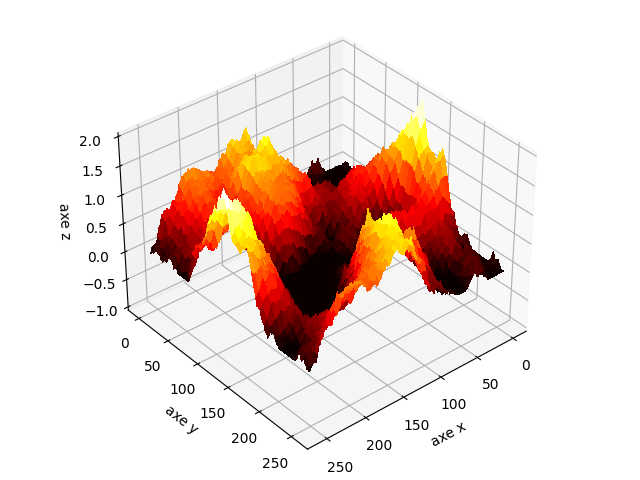
\includegraphics[scale=\myscale,scale=0.4]{figures/diamant-carre-03-2}

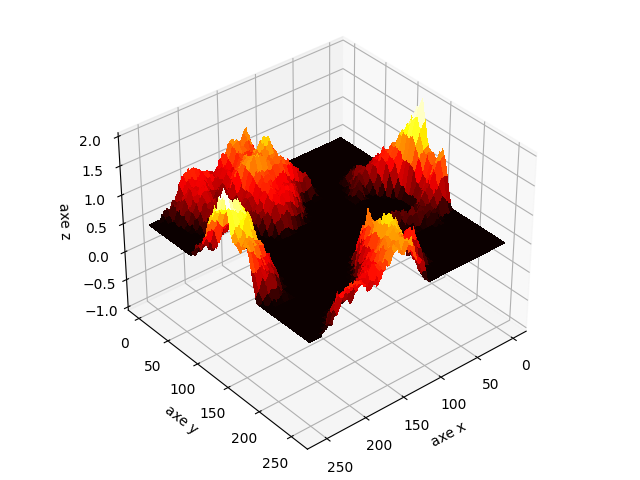
\includegraphics[scale=\myscale,scale=0.4]{figures/diamant-carre-03-3}
\includegraphics[scale=\myscale,scale=0.4]{figures/diamant-carre-03-4}
\end{center}

\end{exemple}


\begin{exemple}
Avec rendu 3D
\begin{center}

\begin{minipage}{0.4\textwidth}
\includegraphics[scale=\myscale,scale=0.5]{figures/hauteurs-04}
\end{minipage}\qquad
\begin{minipage}{0.4\textwidth}
\includegraphics[scale=\myscale,scale=0.5]{figures/hauteurs-05}
\end{minipage}

\smallskip

\includegraphics[scale=\myscale,scale=0.25]{figures/hauteurs-render-new-02}

\smallskip

\nopagebreak

\begin{minipage}{0.8\textwidth}
\center\emph{
(a) La visualisation \Python{} avec \matplotlib.
(b) L'image en niveaux de gris (\emph{heightmap}).
(c) Rendu 3D.}
\end{minipage}

\end{center}


\end{exemple}

%%%%%%%%%%%%%%%%%%%%%%%%%%%%%%%%%%%%%%%%%%%%%%%%%%%%%%%%%%%%%%%%%%%%%
\section{IFS}

\index{fractale!IFS}

%--------------------------------------------------------------------
\subsection{La fougère de Barnsley}

Les IFS (pour \emph{Iterated Functions System}) sont des fractales que l'on trace point par point. Elles permettent de dessiner très facilement des figures géométriques comme le triangle de Sierpinski, mais aussi des objets de la nature, en particulier des feuilles comme la fougère de Barnsley.


\begin{center}

\begin{minipage}{0.4\textwidth}
\includegraphics[scale=\myscale,scale=0.4,trim={1cm 0 1cm 0},clip]{figures/ifs-02}
\end{minipage}\quad
\begin{minipage}{0.3\textwidth}
\includegraphics[scale=\myscale,scale=0.6,trim={5cm 0 5cm 0},clip]{figures/ifs-01}
\end{minipage}

\end{center}

Ce qui est surprenant, c'est que ces dessins sont obtenus par un processus aléatoire et  nécessitent très peu de données, par exemple la fougère est dessinée à partir de $24$ nombres réels seulement.
 

%--------------------------------------------------------------------
\subsection{Transformations du plan}

C'est le moment d'aller relire la section \og{}Transformations du plan\fg{} du chapitre \og{}Matrices\fg{}. On rappelle juste ici la définition générale.

Une \defi{transformation affine}\index{transformation!affine} du plan est l'application $F : \Rr^2 \to \Rr^2$ définie par :
$$
\begin{pmatrix}x \\ y \end{pmatrix} \mapsto \begin{pmatrix}a & b \\ c & d \\  \end{pmatrix}
\begin{pmatrix}x \\ y \end{pmatrix} +\begin{pmatrix} e \\ f \end{pmatrix},$$
où $a,b,c,d, e, f$ sont des réels quelconques.

En d'autres termes, l'image d'un point $(x,y)$ du plan
est le point $F(x,y) = (x',y')$ avec
$$\left \{
\begin{array}{rcl}
    x' &=& ax + by + e \\
    y' &=& cx + dy + f \\
\end{array}
\right..$$

En fait, une transformation affine $F$ est la composée d'une transformation
linéaire 
$$
\begin{pmatrix}x \\ y \end{pmatrix} \mapsto A \begin{pmatrix}x \\ y \end{pmatrix} \qquad \text{ où } \  A =\begin{pmatrix}a & b \\ c & d \\  \end{pmatrix}$$
suivie d'une translation 
$$
\begin{pmatrix}x \\ y \end{pmatrix} \mapsto \begin{pmatrix}x \\ y \end{pmatrix} + B  \qquad \text{ où } \ B =\begin{pmatrix} e \\ f \\  \end{pmatrix}.$$




%--------------------------------------------------------------------
\subsection{Algorithme}

La fractale associée à un système itéré de fonctions s'appelle un \defi{attracteur}.
Comment tracer l'attracteur d'un système itéré de fonctions ?
Soient $F_1,F_2,\ldots,F_\ell$ des transformations affines. 
La méthode la plus efficace afin de tracer la fractale est appelée \og{}jeu du chaos\fg{} :
partant d'un point quelconque $P_0 \in \Rr^2$, on construit une suite de points par récurrence.
Si $P_k$ est construit, alors on choisit aléatoirement l'une des transformations
$F_i$ et on définit $P_{k+1}=F_i(P_k)$. 
On laisse de côté les premiers points (disons les $100$ premiers qui peuvent être \og loin \fg{} de l'attracteur) et on trace les points suivants.

\begin{algorithme}
\textbf{Algorithme \og jeu du chaos \fg{}.}

\textbf{Entrée :} une famille $\{ F_1, F_2,\ldots,F_\ell \}$ de transformations affines.

\textbf{Sortie :} un tracé approché de la fractale.

\begin{itemize}
  \item Fixer $P_0 \in \Rr^2$ au hasard.
    
  \item Pour $k \in \{0,\ldots,N_{\max}\}$ :
  \begin{itemize}
      \item on choisit au hasard $i \in \{1,\ldots,\ell\}$,
      \item on pose $P_{k+1} = F_i(P_k)$,
      \item à partir de $k \ge N_{\min}$ on affiche ce point.
  \end{itemize}
\end{itemize}
\end{algorithme}

$N_{\max}$ représente le nombre de points à calculer (par exemple $N_{\max} = 10\,000$).
$N_{\min}$ est une constante (par exemple $N_{\min} = 100$) qui permet de ne pas tracer les tout premiers points qui peuvent être loin de l'attracteur.


\textbf{Probabilités.}
En plus, pour optimiser les calculs, on ne choisit pas toujours les transformations $F_i$ de façon équiprobable mais avec une probabilité $p_i$ où $p_1+p_2+\cdots+p_\ell=1$. 


%Cette probabilité $p_i$ correspond à la surface couverte par $f_i(C)$ par rapport à celle couverte par $C$. Voici les probabilités pour la fougère de Barnsley : par exemple, la transformation
%$f_1$ qui correspond à un bout de la tige n'est choisie que dans $1\%$ des cas, alors que la transformation
%$f_2$ est choisie dans $85\%$ des cas...



%--------------------------------------------------------------------
\subsection{Exemples}


\textbf{Le triangle de Sierpinski.}

\begin{center}
\includegraphics[scale=\myscale,scale=0.4]{figures/ifs-02}
\end{center}

Voici les valeurs numériques (approchées) qui définissent cette fractale.
\begin{displaymath}
\begin{array}{c|ccccccc}
     & a & b & c & d & e & f & p\\
\hline
F_1 & 0.5 & 0 & 0 & 0.5 & 0 & 0 & 0.33\\
\hline
F_2 & 0.5 & 0 & 0 & 0.5 & 0.5 & 0 & 0.33 \\
\hline
F_3 & 0.5 & 0 & 0 & 0.5 & 0.25 & 0.43 & 0.33 \\
\end{array}
\end{displaymath}

Pour vraiment comprendre l'action des trois fonctions, partons d'un triangle équilatéral $S_0$ dont les sommets sont $(0,0)$,
$(1,0)$, $(\frac12,\frac{\sqrt3}{2})$. On considère les trois transformations affines suivantes :
$$F_1 \begin{pmatrix}x \\ y \end{pmatrix} = \frac12 \begin{pmatrix}x \\ y \end{pmatrix} \qquad
F_2\begin{pmatrix}x \\ y \end{pmatrix} = \frac12 \begin{pmatrix}x \\ y \end{pmatrix}+ \begin{pmatrix} \frac12 \\ 0 \end{pmatrix} \qquad
F_3\begin{pmatrix}x \\ y \end{pmatrix} = \frac12 \begin{pmatrix}x \\ y \end{pmatrix}+ \begin{pmatrix}\frac14 \\ \frac{\sqrt3}{4} \end{pmatrix}
$$

Chacune des transformations $F_i$ est la composition d'une homothétie de rapport $\frac12$ et d'une translation.
\`A la première étape, chacune envoie donc le grand triangle équilatéral $S_0$ sur un triangle plus petit.
Géométriquement, c'est comme si on retirait un triangle au centre de chaque plus gros triangle.
On a représenté $S_0$, $S_1$, $S_2$, $S_3$ et $S_6$, ce qui donne une bonne idée
de l'attracteur, appelé le \defi{triangle de Sierpinski}.

\commentfigure{
\myfigure{1}{\tikzinput{fig_ifs-sierp01}}
}

\bigskip

\textbf{La fougère de Barnsley.}

\begin{center}
\includegraphics[scale=\myscale,scale=0.8]{figures/ifs-01}
\end{center}

\begin{displaymath}
\begin{array}{c|ccccccc}
     & a & b & c & d & e & f & p\\
\hline
F_1 & 0 & 0 & 0 & 0.16 & 0 & 0 & 0.01\\
\hline
F_2  & 0.85 &0.04&-0.04&0.85&0&1.6 & 0.85 \\
\hline
F_3 & 0.2 & -0.26 & 0.23 & 0.22 & 0 & 1.6 & 0.07 \\
\hline
F_4  & -0.15 & 0.28 & 0.26 & 0.24 & 0 & 0.44 & 0.07 \\
\end{array}
\end{displaymath}

\medskip

De part la nature itérative de la construction il est difficile de comprendre ce que fait chaque transformation. Par exemple, la première transformation $F_1$ est une projection composée avec une homothétie d'un petit rapport. Elle envoie toute la fougère sur la base de la tige (la portion verticale).

%
%Voici une explication de chacune des transformations. 
%\begin{itemize}
%  \item La première transformation $F_1$ est une projection composée avec une homothétie d'un petit rapport. Elle envoie toute la fougère sur la base de la tige (la portion verticale).
%  \item La seconde transformation $F_2$ transforme la fougère en la partie supérieure de la fougère (tout sauf les branches droite et gauche les plus basses).
%  \item La transformation $F_3$ envoie la fougère sur la branche basse de droite.
%  \item La transformation $F_4$ envoie la fougère sur la branche basse de gauche.  
%\end{itemize}

\bigskip

\textbf{Autres exemples.}

D'autres formes de feuilles.
\begin{center}
\includegraphics[scale=\myscale,scale=0.6]{figures/ifs-03}
\end{center}

\begin{center}
\includegraphics[scale=\myscale,scale=0.6]{figures/ifs-04}
\end{center}

\begin{center}
\includegraphics[scale=\myscale,scale=0.6]{figures/ifs-05}
\end{center}

Un hippocampe (?). 
\begin{center}
\includegraphics[scale=\myscale,scale=0.6]{figures/ifs-06}
\end{center}

Ci-dessous un exemple d'application du \og{}théorème de collage\fg{} qui permet d'approcher n'importe quel ensemble voulu comme attracteur d'un système itéré de fonctions.
\begin{center}
\includegraphics[scale=\myscale,scale=0.6]{figures/ifs-07}
\end{center}


%%%%%%%%%%%%%%%%%%%%%%%%%%%%%%%%%%%%%%%%%%%%%%%%%%%%%%%%%%%%%%%%%%%%%
\section{L-systèmes}

\index{fractale!L-systeme@L-système}

Les L-systèmes ont été inventés par le botaniste A.~Lindenmayer afin de modéliser les plantes. 
À partir d'un mot initial et d'opérations de remplacement, on arrive à des mots compliqués. Lorsque l'on \og{}dessine\fg{} ces mots, on obtient de superbes figures fractales.


%--------------------------------------------------------------------
\subsection{Tortue}

La \og{}tortue\fg{} est un langage simple pour dessiner : une tortue se déplace dans le plan (ou l'espace) et trace un trait sur son passage. Elle exécute les instructions selon une suite de lettres :


\begin{itemize}
  \item \mot{F} ou \mot{G} : avance d'une quantité fixée (en traçant, \mot{F} pour \emph{forward}),
  \item \mot{+} : tourne à gauche, sans avancer, d'un angle fixé (le plus souvent $\ang{90}$),
  \item \mot{-} : tourne à droite d'un angle fixé.
  \item \mot{[} : mémorise la position de la tortue (coordonnées $(x,y)$ et direction).
  \item \mot{]} : repart de la position mémorisée par le crochet \mot{[} correspondant.
  \item \mot{X}, \mot{Y} : ne font rien. 
\end{itemize}


\begin{exemple}
Comprenons l'exemple du tracé du 
\mot{
{\color{blue}F+F}
{\color{red}[+FFF]}
{\color{green!70!black}F}
{\color{purple}[-FF]}
{\color{orange}F}
}. 
\myfigure{1}{
\tikzinput{fig-crochets}
}    
\begin{itemize}
  \item \mot{{\color{blue}F+F}} : on part du point $O$, on avance, on tourne, on avance.
  \item \mot{{\color{red}[+FFF]}} : on retient la position actuelle (le point $P$) et aussi la direction ; on tourne, on avance trois fois (on trace le segment rouge) ; à la fin on replace la tortue à la position $P$ (sans tracer et avec la même direction que celle auparavant).
  \item \mot{{\color{green!70!black}F}} : depuis $P$ on avance (segment vert).
  \item \mot{{\color{purple}[-FF]}} : on retient la position $Q$ et la direction, on tourne et on trace le segment violet. On revient en $Q$ avec l'ancienne direction.
  \item \mot{{\color{orange}F}} : depuis $Q$ on trace le dernier segment.
\end{itemize}
\end{exemple}


\begin{exercicecours}
Programmer une fonction qui, en entrée reçoit une chaîne de caractères, et trace les instructions correspondantes.

\emph{Indications.}
Avec \Python{} il existe une librairie \ci{turtle} qui fournit les instruction \ci{forward()}, \ci{left()}, \ci{right()}.

\emph{Pile.}
Il est beaucoup plus délicat de gérer les crochets ! La méthode qui rend les choses très simples est d'utiliser une \og{}pile\fg{} (concept que l'on n'expliquera pas ici). 
  \begin{itemize}
    \item Au départ la pile est vide.
	\item On lit un par un les caractères du mot.
	\item Si le caractère est le crochet ouvrant \og{}\mot{[}\fg{} alors on ajoute à la pile la position et la direction courante de la tortue $\big( (x,y), \theta\big)$ (que l'on obtient par \ci{(position(), heading())} du module \ci{turtle}).
	
	\item Si le caractère est le crochet fermant \og{}\mot{]}\fg{} alors on dépile
	(dépiler c'est lire l'élément du haut de la pile et le retirer). On met la position de la tortue et l'angle avec les valeurs lues (utiliser \ci{goto()} et \ci{setheading()}).
	
	\end{itemize}
\end{exercicecours}

%--------------------------------------------------------------------
\subsection{Chercher--Remplacer--Itérer}


Un \defi{L-système} est la donnée d'un mot initial et de règles de remplacement.
Voici un exemple avec le mot de départ et une seule règle : 
\mycenterline{initialisation : \mot{G+F-G} \qquad règle : \mot{F} $\rightarrow$ \mot{FGF}}


Le \defi{$k$-ème itéré} du L-système s'obtient en appliquant $k$ fois la substitution au mot de départ.
Avec notre exemple :
\begin{itemize}
  \item Première itération. Le mot de départ est \mot{G+F-G}, la règle est \mot{F} $\rightarrow$ \mot{FGF} : on remplace le \mot{F} par \mot{FGF}. On obtient le mot \mot{G+FGF-G}.
  
  \item Deuxième itération. On part du mot obtenu \mot{G+FGF-G}, on remplace les deux \mot{F} par \mot{FGF} : on obtient le mot \mot{G+FGFGFGF-G}.
  
  \item Le troisième itéré est \mot{G+FGFGFGFGFGFGFGF-G}, etc.  
\end{itemize}

Lorsqu'il y a deux règles (ou plus) il faut les appliquer en même temps.
Voici un exemple de L-système à deux règles :
\mycenterline{initialisation : \mot{F} \qquad règle 1 : \mot{F} $\rightarrow$ \mot{G+F} \qquad règle 2 : \mot{G} $\rightarrow$ \mot{GG}}
Avec notre exemple :
\begin{itemize}
  \item Première itération. Le mot de départ est \mot{F}, on applique la première règle \mot{F} $\rightarrow$ \mot{G+F} (la seconde règle ne s'applique pas, car il n'y a pas encore de \mot{G}): on obtient le mot \mot{G+F}.
  
  \item Deuxième itération. On part du mot obtenu \mot{G+F}, on remplace le \mot{F} par \mot{G+F} et en même temps le \mot{G} par \mot{GG} : on obtient le mot \mot{GG+G+F}.
  
  \item Le troisième itéré est \mot{GGGG+GG+G+F}, etc.  
\end{itemize}


\begin{exemple}
Considérons le L-système du flocon de Koch :
\mycenterline{initialisation : \mot{F} \qquad règle : \mot{F} $\rightarrow$ \mot{F+F-F-F+F}}
  \begin{itemize}
    \item le premier itéré ($k = 1$) est \mot{F+F-F-F+F}.
    \item le deuxième itéré ($k = 2$) est  :  
     \mycenterline{\mot{F+F-F-F+F+F+F-F-F+F-F+F-F-F+F-F+F-F-F+F+F+F-F-F+F}}
     
    \item avec le troisième itéré ($k = 3$), on obtient \mot{F+F-F-F+F+...} un mot de $249$ lettres.
    
  \end{itemize}
  
 
  Voici les images pour $k=1$ jusqu'à $k=5$ qui correspondent aux premières étapes d'un flocon de Koch.
  
\begin{center}
\includegraphics[scale=\myscale,scale=0.22]{figures/ecran-lsysteme-3a}
\includegraphics[scale=\myscale,scale=0.22]{figures/ecran-lsysteme-3b}
\includegraphics[scale=\myscale,scale=0.22]{figures/ecran-lsysteme-3c}
\includegraphics[scale=\myscale,scale=0.22]{figures/ecran-lsysteme-3d}
\includegraphics[scale=\myscale,scale=0.22]{figures/ecran-lsysteme-3e}
\end{center}
\end{exemple}

\begin{exemple}
Considérons le L-système du triangle de Sierpinski avec deux règles de remplacement :
\mycenterline{initialisation : \mot{F-G-G} \qquad 
règle 1 : \mot{F} $\rightarrow$ \mot{F-G+F+G-F} \qquad
règle 2 : \mot{G} $\rightarrow$ \mot{GG}
}
Par exemple, avec :
  \begin{itemize} 
    \item $k = 1$, \mot{F-G+F+G-F-GG-GG},
    \item pour $k = 2$ :    
    \mycenterline{\mot{F-G+F+G-F-GG+F-G+F+G-F+GG-F-G+F+G-F-GGGG-GGGG}}
  \end{itemize}  

Lorsqu'on trace ces mots (avec un angle de $\ang{-120}$ pour l'instruction \mot{+} et $\ang{120}$ pour l'instruction \mot{-}) on obtient la construction du triangle de Sierpinski. 
  
\begin{center}
\includegraphics[scale=\myscale,scale=0.22]{figures/ecran-lsysteme-7a}
\includegraphics[scale=\myscale,scale=0.22]{figures/ecran-lsysteme-7b}
\includegraphics[scale=\myscale,scale=0.22]{figures/ecran-lsysteme-7c}
\includegraphics[scale=\myscale,scale=0.22]{figures/ecran-lsysteme-7d}
\includegraphics[scale=\myscale,scale=0.22]{figures/ecran-lsysteme-7e}
\end{center}
\end{exemple}

%--------------------------------------------------------------------
\subsection{Plantes en 2D}

Voici des exemples de L-systèmes dont le tracé ressemble à des plantes.
Pour ces exemples, l'angle est généralement fixé à \ang{30}.


% Plante 1 
Voici les quatre premiers tracés du L-système défini par :
\mycenterline{initialisation : \mot{F} \qquad 
règle : \mot{F} $\rightarrow$ \mot{F[+F]F[-F][F]}
}

\begin{center}
\includegraphics[scale=\myscale,scale=0.25]{figures/plante-01-1}
\includegraphics[scale=\myscale,scale=0.25]{figures/plante-01-2}
\includegraphics[scale=\myscale,scale=0.25]{figures/plante-01-3}
\includegraphics[scale=\myscale,scale=0.25]{figures/plante-01-4}
\end{center}


% Plantes 2 et 3
Ci-dessous, à gauche :
\mycenterline{initialisation : \mot{F} \qquad 
règle : \mot{F} $\rightarrow$ \mot{F[+F]F[-F]F}
}
Ci-dessous, à droite  :
\mycenterline{initialisation : \mot{F} \qquad 
règle : \mot{F} $\rightarrow$ \mot{FF-[-F+F+F]+[+F-F-F]}
}

\begin{center}
\includegraphics[scale=\myscale,scale=0.3]{figures/plante-02}\qquad\qquad
\includegraphics[scale=\myscale,scale=0.3]{figures/plante-03}
\end{center}




\begin{center}
\includegraphics[scale=\myscale,scale=0.3]{figures/plante-04}\qquad
\includegraphics[scale=\myscale,scale=0.3]{figures/plante-05}\qquad
\includegraphics[scale=\myscale,scale=0.3]{figures/plante-06}
\end{center}

De gauche à droite :

\begin{center}
\begin{tabular}{lll}
% Plante 4
initialisation : \mot{F} & 
règle 1 : \mot{F} $\rightarrow$ \mot{F[-G][+G]} & 
règle 2 : \mot{G} $\rightarrow$ \mot{F[-G]F[+F-G]}
\\
% Plante 5
initialisation : \mot{YYY} &
règle 1 : \mot{X} $\rightarrow$ \mot{X[-FFF][+FFF]FX} &
règle 2 : \mot{Y} $\rightarrow$ \mot{YFX[+Y][-Y]}
\\
% Plante 6
initialisation : \mot{X} &
règle 1 : \mot{X} $\rightarrow$ \mot{F[+X]F[-X]+X} &
règle 2 : \mot{F} $\rightarrow$ \mot{FF}
\end{tabular}
\end{center}


%--------------------------------------------------------------------
\subsection{Plantes en 3D}

%-----
\subsubsection*{Tortue 3D}

\index{rotation!lacet}
\index{rotation!tangage}
\index{rotation!roulis}

Souvenez-vous des trois mouvements de rotation possibles \emph{yaw/pitch/roll} d'un objet de l'espace, par exemple un avion :
\begin{itemize}
  \item lacet/\emph{yaw} : rotation autour d'un axe haut/bas (un angle positif déplace le nez de l'appareil vers la gauche).	
  \item tangage/\emph{pitch} : rotation autour de l'axe des ailes (un angle positif monte le nez de l'appareil),
  \item roulis/\emph{roll} : rotation autour de l'axe de la cabine (un angle positif fait monter l'aile gauche et baisser l'aile droite).
\end{itemize}


\myfigure{0.9}{
	\tikzinput{fig-yaw-pitch-roll-02}
} 


Jusqu'ici notre tortue se mouvait dans le plan.
Une tortue de l'espace est caractérisée par la position $(x,y,z)$ de son centre, un vecteur $\vec{u}$ pointant vers l'avant et un vecteur $\vec{v}$ indiquant la gauche de la tortue.
Le vecteur $\vec{w} = \vec{u} \wedge \vec{v}$, dirigé vers le haut, complète ces vecteurs en un repère orthonormal direct.

\myfigure{1}{
	\tikzinput{fig-turtle3d}
} 


On étend le langage de la tortue afin qu'elle puisse se déplacer dans l'espace :
  \begin{itemize}
  \item \mot{F} ou \mot{G} : avance d'une quantité fixée,
  \item \mot{+} : tourne vers la gauche, sans avancer, d'un angle fixé (lacet à gauche).
  \item \mot{-} : tourne vers la droite d'un angle fixé (lacet à droite).
  \item \mot{\&} : baisse le nez d'un angle fixé (tangage vers le bas).
  \item \mot{\textasciicircum} : monte le nez d'un angle fixé (tangage vers le haut).
  \item \mot{<} : effectue un roulis vers la gauche d'un angle fixé.
  \item \mot{>} : effectue un roulis vers la droite d'un angle fixé.
  \item \mot{|} : fait demi-tour (lacet de \ang{180}).
  \item \mot{[} : mémorise la position de la tortue (coordonnées $(x,y,z)$ et vecteurs $\vec{u}$ et $\vec{v}$).
  \item \mot{]} : repart de la position mémorisée par le crochet \mot{[} correspondant.
  \item \mot{X}, \mot{Y} : ne font rien. 
\end{itemize}
 

%-----
\subsubsection*{L-système 3D}

\begin{center}
\includegraphics[scale=\myscale,scale=0.6]{figures/plante-01-0}
\end{center}

Considérons le L-système :
\mycenterline{initialisation : \mot{F} \qquad 
règle : \mot{F} $\rightarrow$ \mot{F[\&+F]F[->F]F[+\textasciicircum{}F]F}
}
L'angle est $\frac\pi8$.

Voici les tracés des trois premières itérations.
\begin{center}
\includegraphics[scale=\myscale,scale=0.3]{figures/plante3d-01-1}\qquad
\includegraphics[scale=\myscale,scale=0.3]{figures/plante3d-01-2}\qquad
\includegraphics[scale=\myscale,scale=0.3]{figures/plante3d-01-3}
\end{center}

Voici un autre exemple avec deux vues différentes.
\begin{center}
\includegraphics[scale=\myscale,scale=0.5]{figures/plante3d-02-1}\qquad
\includegraphics[scale=\myscale,scale=0.5]{figures/plante3d-02-2}
\end{center}

Des améliorations sont possibles pour aller plus loin dans le réalisme :
\begin{itemize}
  \item ajouter une texture et des couleurs,
  \item diminuer le diamètre et la longueur des branches au fur et à mesure des itérations,
  \item ajouter des feuilles au bout de chaque branche terminale,
  \item faire une version stochastique c'est-à-dire décider aléatoirement si une branche doit être dessinée ou pas.
\end{itemize}


%-----
\subsubsection*{Courbe de Hilbert 3D}

\index{courbe!de Hilbert}

\begin{center}
\includegraphics[scale=\myscale,scale=0.6]{figures/hilbert-0}
\end{center}

Terminons par une courbe continue de l'espace qui remplit complètement le cube unité. Cette courbe peut être approchée par les itérés du L-système :
\mycenterline{initialisation : \mot{X} \qquad 
règle : \mot{X} $\rightarrow$ \mot{\textasciicircum{}<XF\textasciicircum{}<XFX-F\textasciicircum{}>{}>XFX\&F+>{}>XFX-F>X->}
}
L'angle est $\frac\pi2$.


\begin{center}
\includegraphics[scale=\myscale,scale=0.4]{figures/hilbert-1}\qquad
\includegraphics[scale=\myscale,scale=0.4]{figures/hilbert-2}\qquad

\includegraphics[scale=\myscale,scale=0.4]{figures/hilbert-3}\qquad
\includegraphics[scale=\myscale,scale=0.4]{figures/hilbert-4}
\end{center}

Cela peut être utile si un personnage ou un robot doit inspecter de près chaque point du volume d'une pièce.


\bigskip

Certains paragraphes sont extraits d'un chapitre
\og{}Systèmes itérés de fonctions\fg{} d'un cours de géométrie, d'autres du chapitre 
\og{}L-système\fg{} du livre \og{}Python au lycée\fg{} dans lesquels vous trouverez plus de détails.
Vous trouverez sur notre site une librairie \ci{turtle3d} afin de tracer vos L-systèmes en dimension $3$.

\end{document}
